\documentclass[usenames,dvipsnames]{beamer}
\usepackage[utf8]{inputenc}
\usepackage[english]{babel}
\usepackage{graphicx}
\usepackage{tikz}
\usepackage{amsmath}
\usepackage{amsthm}
\usepackage{amssymb}
\usepackage{mathtools}
\usepackage{csquotes}
\usepackage{tabularx,pbox}
% tikz packages
\usetikzlibrary{positioning}
\usepackage{physics}
\usepackage{yhmath}
\usepackage{cancel}
\usepackage{color}
\usepackage{siunitx}
\usepackage{array}
\usepackage{multirow}
\usepackage{gensymb}
\usepackage{tabularx}
\usepackage{extarrows}
\usepackage{booktabs}
\usetikzlibrary{fadings}
\usetikzlibrary{patterns}
\usetikzlibrary{shadows.blur}
\usetikzlibrary{shapes}

\definecolor{carminepink}{rgb}{0.92, 0.3, 0.26}
\definecolor{candypink}{rgb}{0.89, 0.44, 0.48}

% theme
\usetheme[numbering=counter, progressbar=foot, titleformat=allcaps]{metropolis}  
\setbeamercolor{title separator}{fg=BrickRed}
\setbeamercolor{progress bar in head/foot}{fg=BrickRed}
\setbeamercolor{alerted text}{fg=BrickRed}

\newcommand{\tabitem}{~~\llap{\textbullet}~~}

\title{Markov Chain Analysis of \\The Ehrenfest Urn Model}
\date{2020/2021}
\author{Elena Acinapura}
\institute{Università di Trento}

\begin{document}
  \maketitle
  \section{Motivation}
  \begin{frame}{Irreversibility vs Recurrence}
    Some thermodynamic processes, such as 

    \begin{table}
        \begin{center}
        \begin{tabular}{l c}
            \tabitem diffusions & \\
            \tabitem heat transfers & $\rightarrow \quad $ \alert{irreversible}\\
            \tabitem phase transitions & 
        \end{tabular}
        \end{center}
    \end{table}
    
    \begin{center}
        \textbf{but}
    \end{center}
    
    \begin{center}
    Newtonian mechanics $\quad \rightarrow \quad$ \alert{time-reversible}
    \end{center}
  \end{frame}

  \begin{frame}{Contents}
    \textbf{The Ehrenfest urn model}

    \medskip
    \textbf{Analysis via Markov chains}
      \begin{itemize}
        \item limiting distribution
        \item mean recurrence time
      \end{itemize}
      \medskip
    \textbf{Simulation}
  \end{frame}

  \section{The Ehrenfest Urn Model}
  \begin{frame}{The Ehrenfest Urn Model} %intro
    Diffusion of a gas as \alert{stochastic process}
    \begin{itemize}
      \item $N$ particles
      \item 2 boxes
      \item discretized time steps
    \end{itemize}
   
    \begin{figure}
      \begin{center}
        \input{pictures/ehrenfest_1}
      \end{center}
    \end{figure}

  \end{frame}

  \begin{frame}{The Ehrenfest Urn Model} %select particle
    At each time step:
    \begin{itemize}
      \item \alert{a ball is selected at random among the $N$ possible ones}
    \end{itemize}

    \medskip
    \begin{figure}[b]
      \begin{center}
        \input{pictures/picked_ball}
      \end{center}
    \end{figure}
  \end{frame}

  \begin{frame}{The Ehrenfest Urn Model} %extract particle
    At each time step:
    \begin{itemize}
      \item a ball is selected at random among the $N$ possible ones
      \item \alert{it is extracted from its box}
    \end{itemize}

    \medskip
    \begin{figure}[b]
      \begin{center}
        


\tikzset{every picture/.style={line width=0.75pt}} %set default line width to 0.75pt        

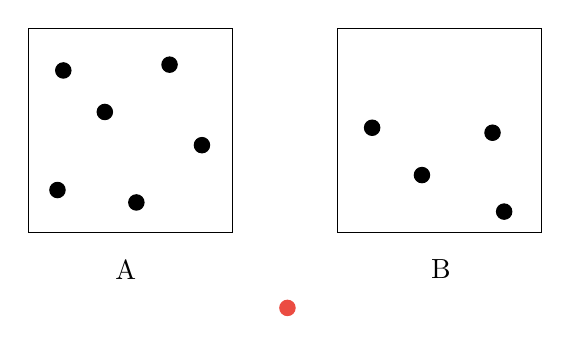
\begin{tikzpicture}[x=0.75pt,y=0.75pt,yscale=-1,xscale=1]
%uncomment if require: \path (0,375); %set diagram left start at 0, and has height of 375

%Shape: Square [id:dp5886506825268709] 
\draw   (181,91.16) -- (279.34,91.16) -- (279.34,189.5) -- (181,189.5) -- cycle ;
%Shape: Square [id:dp24242986167867575] 
\draw   (330,91.16) -- (428.34,91.16) -- (428.34,189.5) -- (330,189.5) -- cycle ;
%Shape: Circle [id:dp48354636802020234] 
\draw  [fill={rgb, 255:red, 0; green, 0; blue, 0 }  ,fill opacity=1 ] (194.19,111.5) .. controls (194.19,109.46) and (195.85,107.8) .. (197.9,107.8) .. controls (199.94,107.8) and (201.6,109.46) .. (201.6,111.5) .. controls (201.6,113.55) and (199.94,115.21) .. (197.9,115.21) .. controls (195.85,115.21) and (194.19,113.55) .. (194.19,111.5) -- cycle ;
%Shape: Circle [id:dp8547166774432848] 
\draw  [fill={rgb, 255:red, 0; green, 0; blue, 0 }  ,fill opacity=1 ] (214.19,131.5) .. controls (214.19,129.46) and (215.85,127.8) .. (217.9,127.8) .. controls (219.94,127.8) and (221.6,129.46) .. (221.6,131.5) .. controls (221.6,133.55) and (219.94,135.21) .. (217.9,135.21) .. controls (215.85,135.21) and (214.19,133.55) .. (214.19,131.5) -- cycle ;
%Shape: Circle [id:dp3635316819967491] 
\draw  [fill={rgb, 255:red, 0; green, 0; blue, 0 }  ,fill opacity=1 ] (191.39,169.1) .. controls (191.39,167.06) and (193.05,165.4) .. (195.1,165.4) .. controls (197.14,165.4) and (198.8,167.06) .. (198.8,169.1) .. controls (198.8,171.15) and (197.14,172.81) .. (195.1,172.81) .. controls (193.05,172.81) and (191.39,171.15) .. (191.39,169.1) -- cycle ;
%Shape: Circle [id:dp504377272845598] 
\draw  [fill={rgb, 255:red, 0; green, 0; blue, 0 }  ,fill opacity=1 ] (245.39,108.7) .. controls (245.39,106.66) and (247.05,105) .. (249.1,105) .. controls (251.14,105) and (252.8,106.66) .. (252.8,108.7) .. controls (252.8,110.75) and (251.14,112.41) .. (249.1,112.41) .. controls (247.05,112.41) and (245.39,110.75) .. (245.39,108.7) -- cycle ;
%Shape: Circle [id:dp40762374287455616] 
\draw  [fill={rgb, 255:red, 0; green, 0; blue, 0 }  ,fill opacity=1 ] (229.39,175.1) .. controls (229.39,173.06) and (231.05,171.4) .. (233.1,171.4) .. controls (235.14,171.4) and (236.8,173.06) .. (236.8,175.1) .. controls (236.8,177.15) and (235.14,178.81) .. (233.1,178.81) .. controls (231.05,178.81) and (229.39,177.15) .. (229.39,175.1) -- cycle ;
%Shape: Circle [id:dp8577561818936912] 
\draw  [fill={rgb, 255:red, 0; green, 0; blue, 0 }  ,fill opacity=1 ] (260.99,147.5) .. controls (260.99,145.46) and (262.65,143.8) .. (264.7,143.8) .. controls (266.74,143.8) and (268.4,145.46) .. (268.4,147.5) .. controls (268.4,149.55) and (266.74,151.21) .. (264.7,151.21) .. controls (262.65,151.21) and (260.99,149.55) .. (260.99,147.5) -- cycle ;
%Shape: Circle [id:dp3598710056160941] 
\draw  [color=carminepink  ,draw opacity=1 ][fill=carminepink  ,fill opacity=1 ] (302.19,225.9) .. controls (302.19,223.86) and (303.85,222.2) .. (305.9,222.2) .. controls (307.94,222.2) and (309.6,223.86) .. (309.6,225.9) .. controls (309.6,227.95) and (307.94,229.61) .. (305.9,229.61) .. controls (303.85,229.61) and (302.19,227.95) .. (302.19,225.9) -- cycle ;
%Shape: Circle [id:dp8070234513651793] 
\draw  [fill={rgb, 255:red, 0; green, 0; blue, 0 }  ,fill opacity=1 ] (342.99,139.1) .. controls (342.99,137.06) and (344.65,135.4) .. (346.7,135.4) .. controls (348.74,135.4) and (350.4,137.06) .. (350.4,139.1) .. controls (350.4,141.15) and (348.74,142.81) .. (346.7,142.81) .. controls (344.65,142.81) and (342.99,141.15) .. (342.99,139.1) -- cycle ;
%Shape: Circle [id:dp3126762302018198] 
\draw  [fill={rgb, 255:red, 0; green, 0; blue, 0 }  ,fill opacity=1 ] (366.99,161.9) .. controls (366.99,159.86) and (368.65,158.2) .. (370.7,158.2) .. controls (372.74,158.2) and (374.4,159.86) .. (374.4,161.9) .. controls (374.4,163.95) and (372.74,165.61) .. (370.7,165.61) .. controls (368.65,165.61) and (366.99,163.95) .. (366.99,161.9) -- cycle ;
%Shape: Circle [id:dp24135298904714841] 
\draw  [fill={rgb, 255:red, 0; green, 0; blue, 0 }  ,fill opacity=1 ] (406.59,179.5) .. controls (406.59,177.46) and (408.25,175.8) .. (410.3,175.8) .. controls (412.34,175.8) and (414,177.46) .. (414,179.5) .. controls (414,181.55) and (412.34,183.21) .. (410.3,183.21) .. controls (408.25,183.21) and (406.59,181.55) .. (406.59,179.5) -- cycle ;
%Shape: Circle [id:dp9432634536780442] 
\draw  [fill={rgb, 255:red, 0; green, 0; blue, 0 }  ,fill opacity=1 ] (400.99,141.5) .. controls (400.99,139.46) and (402.65,137.8) .. (404.7,137.8) .. controls (406.74,137.8) and (408.4,139.46) .. (408.4,141.5) .. controls (408.4,143.55) and (406.74,145.21) .. (404.7,145.21) .. controls (402.65,145.21) and (400.99,143.55) .. (400.99,141.5) -- cycle ;

% Text Node
\draw (221.73,201.87) node [anchor=north west][inner sep=0.75pt]    {$\text{A}$};
% Text Node
\draw (373.8,201.54) node [anchor=north west][inner sep=0.75pt]    {$\text{B}$};


\end{tikzpicture}
      \end{center}
    \end{figure}
  \end{frame}

  \begin{frame}{The Ehrenfest Urn Model} % select box
    At each time step:
    \begin{itemize}
      \item a ball is selected at random among the $N$ possible ones
      \item it is extracted from its box
      \item \alert{a box is selected at random}
    \end{itemize}

    \medskip
    \begin{figure}[b]
      \begin{center}
        \input{pictures/box_selected}
      \end{center}
    \end{figure}
  \end{frame}

  \begin{frame}{The Ehrenfest Urn Model} % put
    At each time step:
    \begin{itemize}
      \item a ball is selected at random among the $N$ possible ones
      \item it is extracted from its box
      \item a box is selected at random
      \item \alert{the particle is put in the selected box}
    \end{itemize}

    \medskip
    \begin{figure}[b]
      \begin{center}
        \input{pictures/put}
      \end{center}
    \end{figure}
  \end{frame}

  \begin{frame}{The Ehrenfest Urn Model}
    \begin{center}
      \textbf{Meaningful questions about equilibrium}
    \end{center}
    \begin{itemize}
      \item probability of having all the particles in box A?
    \end{itemize}
    \begin{figure}
      


\tikzset{every picture/.style={line width=0.75pt}} %set default line width to 0.75pt        

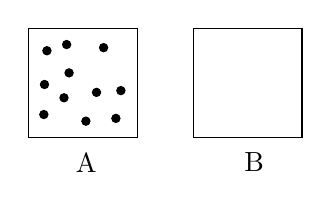
\begin{tikzpicture}[x=0.40,y=0.40,yscale=-1,xscale=1]
    %uncomment if require: \path (0,375); %set diagram left start at 0, and has height of 375

%Shape: Square [id:dp5886506825268709] 
\draw  [color={rgb, 255:red, 0; green, 0; blue, 0 }  ,draw opacity=1 ] (181,91.16) -- (279.34,91.16) -- (279.34,189.5) -- (181,189.5) -- cycle ;
%Shape: Square [id:dp24242986167867575] 
\draw   (330,91.16) -- (428.34,91.16) -- (428.34,189.5) -- (330,189.5) -- cycle ;
%Shape: Circle [id:dp48354636802020234] 
\draw  [fill={rgb, 255:red, 0; green, 0; blue, 0 }  ,fill opacity=1 ] (194.19,111.5) .. controls (194.19,109.46) and (195.85,107.8) .. (197.9,107.8) .. controls (199.94,107.8) and (201.6,109.46) .. (201.6,111.5) .. controls (201.6,113.55) and (199.94,115.21) .. (197.9,115.21) .. controls (195.85,115.21) and (194.19,113.55) .. (194.19,111.5) -- cycle ;
%Shape: Circle [id:dp8547166774432848] 
\draw  [fill={rgb, 255:red, 0; green, 0; blue, 0 }  ,fill opacity=1 ] (214.19,131.5) .. controls (214.19,129.46) and (215.85,127.8) .. (217.9,127.8) .. controls (219.94,127.8) and (221.6,129.46) .. (221.6,131.5) .. controls (221.6,133.55) and (219.94,135.21) .. (217.9,135.21) .. controls (215.85,135.21) and (214.19,133.55) .. (214.19,131.5) -- cycle ;
%Shape: Circle [id:dp3635316819967491] 
\draw  [fill={rgb, 255:red, 0; green, 0; blue, 0 }  ,fill opacity=1 ] (191.39,169.1) .. controls (191.39,167.06) and (193.05,165.4) .. (195.1,165.4) .. controls (197.14,165.4) and (198.8,167.06) .. (198.8,169.1) .. controls (198.8,171.15) and (197.14,172.81) .. (195.1,172.81) .. controls (193.05,172.81) and (191.39,171.15) .. (191.39,169.1) -- cycle ;
%Shape: Circle [id:dp504377272845598] 
\draw  [fill={rgb, 255:red, 0; green, 0; blue, 0 }  ,fill opacity=1 ] (245.39,108.7) .. controls (245.39,106.66) and (247.05,105) .. (249.1,105) .. controls (251.14,105) and (252.8,106.66) .. (252.8,108.7) .. controls (252.8,110.75) and (251.14,112.41) .. (249.1,112.41) .. controls (247.05,112.41) and (245.39,110.75) .. (245.39,108.7) -- cycle ;
%Shape: Circle [id:dp40762374287455616] 
\draw  [fill={rgb, 255:red, 0; green, 0; blue, 0 }  ,fill opacity=1 ] (229.39,175.1) .. controls (229.39,173.06) and (231.05,171.4) .. (233.1,171.4) .. controls (235.14,171.4) and (236.8,173.06) .. (236.8,175.1) .. controls (236.8,177.15) and (235.14,178.81) .. (233.1,178.81) .. controls (231.05,178.81) and (229.39,177.15) .. (229.39,175.1) -- cycle ;
%Shape: Circle [id:dp8577561818936912] 
\draw  [fill={rgb, 255:red, 0; green, 0; blue, 0 }  ,fill opacity=1 ] (260.99,147.5) .. controls (260.99,145.46) and (262.65,143.8) .. (264.7,143.8) .. controls (266.74,143.8) and (268.4,145.46) .. (268.4,147.5) .. controls (268.4,149.55) and (266.74,151.21) .. (264.7,151.21) .. controls (262.65,151.21) and (260.99,149.55) .. (260.99,147.5) -- cycle ;
%Shape: Circle [id:dp3598710056160941] 
\draw  [color={rgb, 255:red, 0; green, 0; blue, 0 }  ,draw opacity=1 ][fill={rgb, 255:red, 0; green, 0; blue, 0 }  ,fill opacity=1 ] (238.99,149.1) .. controls (238.99,147.06) and (240.65,145.4) .. (242.7,145.4) .. controls (244.74,145.4) and (246.4,147.06) .. (246.4,149.1) .. controls (246.4,151.15) and (244.74,152.81) .. (242.7,152.81) .. controls (240.65,152.81) and (238.99,151.15) .. (238.99,149.1) -- cycle ;
%Shape: Circle [id:dp8070234513651793] 
\draw  [fill={rgb, 255:red, 0; green, 0; blue, 0 }  ,fill opacity=1 ] (256.49,172.6) .. controls (256.49,170.56) and (258.15,168.9) .. (260.2,168.9) .. controls (262.24,168.9) and (263.9,170.56) .. (263.9,172.6) .. controls (263.9,174.65) and (262.24,176.31) .. (260.2,176.31) .. controls (258.15,176.31) and (256.49,174.65) .. (256.49,172.6) -- cycle ;
%Shape: Circle [id:dp3126762302018198] 
\draw  [fill={rgb, 255:red, 0; green, 0; blue, 0 }  ,fill opacity=1 ] (211.99,105.9) .. controls (211.99,103.86) and (213.65,102.2) .. (215.7,102.2) .. controls (217.74,102.2) and (219.4,103.86) .. (219.4,105.9) .. controls (219.4,107.95) and (217.74,109.61) .. (215.7,109.61) .. controls (213.65,109.61) and (211.99,107.95) .. (211.99,105.9) -- cycle ;
%Shape: Circle [id:dp24135298904714841] 
\draw  [fill={rgb, 255:red, 0; green, 0; blue, 0 }  ,fill opacity=1 ] (209.59,154) .. controls (209.59,151.96) and (211.25,150.3) .. (213.3,150.3) .. controls (215.34,150.3) and (217,151.96) .. (217,154) .. controls (217,156.05) and (215.34,157.71) .. (213.3,157.71) .. controls (211.25,157.71) and (209.59,156.05) .. (209.59,154) -- cycle ;
%Shape: Circle [id:dp9432634536780442] 
\draw  [fill={rgb, 255:red, 0; green, 0; blue, 0 }  ,fill opacity=1 ] (191.99,142) .. controls (191.99,139.96) and (193.65,138.3) .. (195.7,138.3) .. controls (197.74,138.3) and (199.4,139.96) .. (199.4,142) .. controls (199.4,144.05) and (197.74,145.71) .. (195.7,145.71) .. controls (193.65,145.71) and (191.99,144.05) .. (191.99,142) -- cycle ;

% Text Node
\draw (221.73,201.87) node [anchor=north west][inner sep=0.75pt]    {$\text{A}$};
% Text Node
\draw (373.8,201.54) node [anchor=north west][inner sep=0.75pt]    {$\text{B}$};


\end{tikzpicture}
    \end{figure}
    \begin{itemize}
      \item time needed for recurrence?
    \end{itemize}
    \begin{figure}
      



\tikzset{every picture/.style={line width=0.75pt}} %set default line width to 0.75pt        

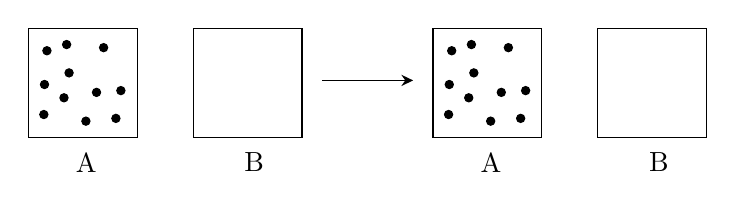
\begin{tikzpicture}[x=0.40,y=0.40,yscale=-1,xscale=1]
%uncomment if require: \path (0,594); %set diagram left start at 0, and has height of 594

%Shape: Square [id:dp774487099896747] 
\draw  [color={rgb, 255:red, 0; green, 0; blue, 0 }  ,draw opacity=1 ] (14.6,103.16) -- (112.94,103.16) -- (112.94,201.5) -- (14.6,201.5) -- cycle ;
%Shape: Square [id:dp025429925890165128] 
\draw   (163.6,103.16) -- (261.94,103.16) -- (261.94,201.5) -- (163.6,201.5) -- cycle ;
%Shape: Circle [id:dp3181813441668684] 
\draw  [fill={rgb, 255:red, 0; green, 0; blue, 0 }  ,fill opacity=1 ] (27.79,123.5) .. controls (27.79,121.46) and (29.45,119.8) .. (31.5,119.8) .. controls (33.54,119.8) and (35.2,121.46) .. (35.2,123.5) .. controls (35.2,125.55) and (33.54,127.21) .. (31.5,127.21) .. controls (29.45,127.21) and (27.79,125.55) .. (27.79,123.5) -- cycle ;
%Shape: Circle [id:dp603908038435023] 
\draw  [fill={rgb, 255:red, 0; green, 0; blue, 0 }  ,fill opacity=1 ] (47.79,143.5) .. controls (47.79,141.46) and (49.45,139.8) .. (51.5,139.8) .. controls (53.54,139.8) and (55.2,141.46) .. (55.2,143.5) .. controls (55.2,145.55) and (53.54,147.21) .. (51.5,147.21) .. controls (49.45,147.21) and (47.79,145.55) .. (47.79,143.5) -- cycle ;
%Shape: Circle [id:dp5952281148881424] 
\draw  [fill={rgb, 255:red, 0; green, 0; blue, 0 }  ,fill opacity=1 ] (24.99,181.1) .. controls (24.99,179.06) and (26.65,177.4) .. (28.7,177.4) .. controls (30.74,177.4) and (32.4,179.06) .. (32.4,181.1) .. controls (32.4,183.15) and (30.74,184.81) .. (28.7,184.81) .. controls (26.65,184.81) and (24.99,183.15) .. (24.99,181.1) -- cycle ;
%Shape: Circle [id:dp8284021424683614] 
\draw  [fill={rgb, 255:red, 0; green, 0; blue, 0 }  ,fill opacity=1 ] (78.99,120.7) .. controls (78.99,118.66) and (80.65,117) .. (82.7,117) .. controls (84.74,117) and (86.4,118.66) .. (86.4,120.7) .. controls (86.4,122.75) and (84.74,124.41) .. (82.7,124.41) .. controls (80.65,124.41) and (78.99,122.75) .. (78.99,120.7) -- cycle ;
%Shape: Circle [id:dp5147293581241896] 
\draw  [fill={rgb, 255:red, 0; green, 0; blue, 0 }  ,fill opacity=1 ] (62.99,187.1) .. controls (62.99,185.06) and (64.65,183.4) .. (66.7,183.4) .. controls (68.74,183.4) and (70.4,185.06) .. (70.4,187.1) .. controls (70.4,189.15) and (68.74,190.81) .. (66.7,190.81) .. controls (64.65,190.81) and (62.99,189.15) .. (62.99,187.1) -- cycle ;
%Shape: Circle [id:dp9005778661722459] 
\draw  [fill={rgb, 255:red, 0; green, 0; blue, 0 }  ,fill opacity=1 ] (94.59,159.5) .. controls (94.59,157.46) and (96.25,155.8) .. (98.3,155.8) .. controls (100.34,155.8) and (102,157.46) .. (102,159.5) .. controls (102,161.55) and (100.34,163.21) .. (98.3,163.21) .. controls (96.25,163.21) and (94.59,161.55) .. (94.59,159.5) -- cycle ;
%Shape: Circle [id:dp1200483422476748] 
\draw  [color={rgb, 255:red, 0; green, 0; blue, 0 }  ,draw opacity=1 ][fill={rgb, 255:red, 0; green, 0; blue, 0 }  ,fill opacity=1 ] (72.59,161.1) .. controls (72.59,159.06) and (74.25,157.4) .. (76.3,157.4) .. controls (78.34,157.4) and (80,159.06) .. (80,161.1) .. controls (80,163.15) and (78.34,164.81) .. (76.3,164.81) .. controls (74.25,164.81) and (72.59,163.15) .. (72.59,161.1) -- cycle ;
%Shape: Circle [id:dp8676035581957091] 
\draw  [fill={rgb, 255:red, 0; green, 0; blue, 0 }  ,fill opacity=1 ] (90.09,184.6) .. controls (90.09,182.56) and (91.75,180.9) .. (93.8,180.9) .. controls (95.84,180.9) and (97.5,182.56) .. (97.5,184.6) .. controls (97.5,186.65) and (95.84,188.31) .. (93.8,188.31) .. controls (91.75,188.31) and (90.09,186.65) .. (90.09,184.6) -- cycle ;
%Shape: Circle [id:dp7565040593219183] 
\draw  [fill={rgb, 255:red, 0; green, 0; blue, 0 }  ,fill opacity=1 ] (45.59,117.9) .. controls (45.59,115.86) and (47.25,114.2) .. (49.3,114.2) .. controls (51.34,114.2) and (53,115.86) .. (53,117.9) .. controls (53,119.95) and (51.34,121.61) .. (49.3,121.61) .. controls (47.25,121.61) and (45.59,119.95) .. (45.59,117.9) -- cycle ;
%Shape: Circle [id:dp5827285696809148] 
\draw  [fill={rgb, 255:red, 0; green, 0; blue, 0 }  ,fill opacity=1 ] (43.19,166) .. controls (43.19,163.96) and (44.85,162.3) .. (46.9,162.3) .. controls (48.94,162.3) and (50.6,163.96) .. (50.6,166) .. controls (50.6,168.05) and (48.94,169.71) .. (46.9,169.71) .. controls (44.85,169.71) and (43.19,168.05) .. (43.19,166) -- cycle ;
%Shape: Circle [id:dp8537532752530581] 
\draw  [fill={rgb, 255:red, 0; green, 0; blue, 0 }  ,fill opacity=1 ] (25.59,154) .. controls (25.59,151.96) and (27.25,150.3) .. (29.3,150.3) .. controls (31.34,150.3) and (33,151.96) .. (33,154) .. controls (33,156.05) and (31.34,157.71) .. (29.3,157.71) .. controls (27.25,157.71) and (25.59,156.05) .. (25.59,154) -- cycle ;

%Shape: Square [id:dp47379006085778586] 
\draw  [color={rgb, 255:red, 0; green, 0; blue, 0 }  ,draw opacity=1 ] (380.27,103.16) -- (478.61,103.16) -- (478.61,201.5) -- (380.27,201.5) -- cycle ;
%Shape: Square [id:dp2821189539464646] 
\draw   (529.27,103.16) -- (627.61,103.16) -- (627.61,201.5) -- (529.27,201.5) -- cycle ;
%Shape: Circle [id:dp9518174840357838] 
\draw  [fill={rgb, 255:red, 0; green, 0; blue, 0 }  ,fill opacity=1 ] (393.46,123.5) .. controls (393.46,121.46) and (395.12,119.8) .. (397.16,119.8) .. controls (399.21,119.8) and (400.87,121.46) .. (400.87,123.5) .. controls (400.87,125.55) and (399.21,127.21) .. (397.16,127.21) .. controls (395.12,127.21) and (393.46,125.55) .. (393.46,123.5) -- cycle ;
%Shape: Circle [id:dp10416646358549686] 
\draw  [fill={rgb, 255:red, 0; green, 0; blue, 0 }  ,fill opacity=1 ] (413.46,143.5) .. controls (413.46,141.46) and (415.12,139.8) .. (417.16,139.8) .. controls (419.21,139.8) and (420.87,141.46) .. (420.87,143.5) .. controls (420.87,145.55) and (419.21,147.21) .. (417.16,147.21) .. controls (415.12,147.21) and (413.46,145.55) .. (413.46,143.5) -- cycle ;
%Shape: Circle [id:dp5588791845696657] 
\draw  [fill={rgb, 255:red, 0; green, 0; blue, 0 }  ,fill opacity=1 ] (390.66,181.1) .. controls (390.66,179.06) and (392.32,177.4) .. (394.36,177.4) .. controls (396.41,177.4) and (398.07,179.06) .. (398.07,181.1) .. controls (398.07,183.15) and (396.41,184.81) .. (394.36,184.81) .. controls (392.32,184.81) and (390.66,183.15) .. (390.66,181.1) -- cycle ;
%Shape: Circle [id:dp8513830063391616] 
\draw  [fill={rgb, 255:red, 0; green, 0; blue, 0 }  ,fill opacity=1 ] (444.66,120.7) .. controls (444.66,118.66) and (446.32,117) .. (448.36,117) .. controls (450.41,117) and (452.07,118.66) .. (452.07,120.7) .. controls (452.07,122.75) and (450.41,124.41) .. (448.36,124.41) .. controls (446.32,124.41) and (444.66,122.75) .. (444.66,120.7) -- cycle ;
%Shape: Circle [id:dp5926273769306261] 
\draw  [fill={rgb, 255:red, 0; green, 0; blue, 0 }  ,fill opacity=1 ] (428.66,187.1) .. controls (428.66,185.06) and (430.32,183.4) .. (432.36,183.4) .. controls (434.41,183.4) and (436.07,185.06) .. (436.07,187.1) .. controls (436.07,189.15) and (434.41,190.81) .. (432.36,190.81) .. controls (430.32,190.81) and (428.66,189.15) .. (428.66,187.1) -- cycle ;
%Shape: Circle [id:dp9762739798450286] 
\draw  [fill={rgb, 255:red, 0; green, 0; blue, 0 }  ,fill opacity=1 ] (460.26,159.5) .. controls (460.26,157.46) and (461.92,155.8) .. (463.96,155.8) .. controls (466.01,155.8) and (467.67,157.46) .. (467.67,159.5) .. controls (467.67,161.55) and (466.01,163.21) .. (463.96,163.21) .. controls (461.92,163.21) and (460.26,161.55) .. (460.26,159.5) -- cycle ;
%Shape: Circle [id:dp8228034661014085] 
\draw  [color={rgb, 255:red, 0; green, 0; blue, 0 }  ,draw opacity=1 ][fill={rgb, 255:red, 0; green, 0; blue, 0 }  ,fill opacity=1 ] (438.26,161.1) .. controls (438.26,159.06) and (439.92,157.4) .. (441.96,157.4) .. controls (444.01,157.4) and (445.67,159.06) .. (445.67,161.1) .. controls (445.67,163.15) and (444.01,164.81) .. (441.96,164.81) .. controls (439.92,164.81) and (438.26,163.15) .. (438.26,161.1) -- cycle ;
%Shape: Circle [id:dp2750535519586872] 
\draw  [fill={rgb, 255:red, 0; green, 0; blue, 0 }  ,fill opacity=1 ] (455.76,184.6) .. controls (455.76,182.56) and (457.42,180.9) .. (459.46,180.9) .. controls (461.51,180.9) and (463.17,182.56) .. (463.17,184.6) .. controls (463.17,186.65) and (461.51,188.31) .. (459.46,188.31) .. controls (457.42,188.31) and (455.76,186.65) .. (455.76,184.6) -- cycle ;
%Shape: Circle [id:dp9526778939911018] 
\draw  [fill={rgb, 255:red, 0; green, 0; blue, 0 }  ,fill opacity=1 ] (411.26,117.9) .. controls (411.26,115.86) and (412.92,114.2) .. (414.96,114.2) .. controls (417.01,114.2) and (418.67,115.86) .. (418.67,117.9) .. controls (418.67,119.95) and (417.01,121.61) .. (414.96,121.61) .. controls (412.92,121.61) and (411.26,119.95) .. (411.26,117.9) -- cycle ;
%Shape: Circle [id:dp3752188484747254] 
\draw  [fill={rgb, 255:red, 0; green, 0; blue, 0 }  ,fill opacity=1 ] (408.86,166) .. controls (408.86,163.96) and (410.52,162.3) .. (412.56,162.3) .. controls (414.61,162.3) and (416.27,163.96) .. (416.27,166) .. controls (416.27,168.05) and (414.61,169.71) .. (412.56,169.71) .. controls (410.52,169.71) and (408.86,168.05) .. (408.86,166) -- cycle ;
%Shape: Circle [id:dp8850820592925885] 
\draw  [fill={rgb, 255:red, 0; green, 0; blue, 0 }  ,fill opacity=1 ] (391.26,154) .. controls (391.26,151.96) and (392.92,150.3) .. (394.96,150.3) .. controls (397.01,150.3) and (398.67,151.96) .. (398.67,154) .. controls (398.67,156.05) and (397.01,157.71) .. (394.96,157.71) .. controls (392.92,157.71) and (391.26,156.05) .. (391.26,154) -- cycle ;

%Straight Lines [id:da9001462483621545] 
\draw    (280,150.3) -- (359.33,150.3) ;
\draw [shift={(362.33,150.3)}, rotate = 180] [fill={rgb, 255:red, 0; green, 0; blue, 0 }  ][line width=0.08]  [draw opacity=0] (10.72,-5.15) -- (0,0) -- (10.72,5.15) -- (7.12,0) -- cycle    ;

% Text Node
\draw (573.07,213.54) node [anchor=north west][inner sep=0.75pt]    {$\text{B}$};
% Text Node
\draw (421,213.87) node [anchor=north west][inner sep=0.75pt]    {$\text{A}$};
% Text Node
\draw (207.4,213.54) node [anchor=north west][inner sep=0.75pt]    {$\text{B}$};
% Text Node
\draw (55.33,213.87) node [anchor=north west][inner sep=0.75pt]    {$\text{A}$};


\end{tikzpicture}
    \end{figure}
  \end{frame}

  \section{Markov chain analysis}
  \begin{frame}{Markov chains - definition}
    \begin{center}
      \textbf{Discrete Markov chains}
    \end{center}
    A mathematical theory for stochastic processes
    \begin{figure}
      


\tikzset{every picture/.style={line width=0.75pt}} %set default line width to 0.75pt        

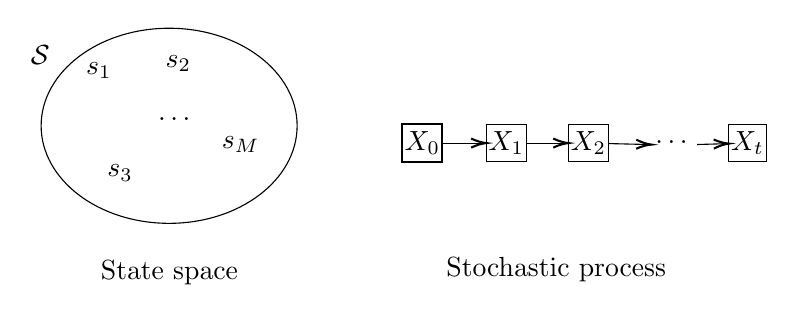
\begin{tikzpicture}[x=0.50pt,y=0.50pt,yscale=-1,xscale=1]
%uncomment if require: \path (0,928); %set diagram left start at 0, and has height of 928

%Shape: Ellipse [id:dp18659796531361872] 
\draw   (59.33,412.31) .. controls (59.33,373.38) and (100.75,341.81) .. (151.83,341.81) .. controls (202.92,341.81) and (244.33,373.38) .. (244.33,412.31) .. controls (244.33,451.25) and (202.92,482.81) .. (151.83,482.81) .. controls (100.75,482.81) and (59.33,451.25) .. (59.33,412.31) -- cycle ;

% Text Node
\draw (50,352.15) node [anchor=north west][inner sep=0.75pt]    {$\mathcal{S}$};
% Text Node
\draw (100.67,507.81) node [anchor=north west][inner sep=0.75pt]   [align=left] {State space};
% Text Node
\draw (90,364.48) node [anchor=north west][inner sep=0.75pt]    {$s_{1}$};
% Text Node
\draw (147.33,359.81) node [anchor=north west][inner sep=0.75pt]    {$s_{2}$};
% Text Node
\draw (105.33,438.81) node [anchor=north west][inner sep=0.75pt]    {$s_{3}$};
% Text Node
\draw (142,404.15) node [anchor=north west][inner sep=0.75pt]    {$\dotsc $};
% Text Node
\draw (188,418.15) node [anchor=north west][inner sep=0.75pt]    {$s_{M}$};
% Text Node
\draw  [line width=0.75]   (320.36,411.31) -- (349.36,411.31) -- (349.36,438.31) -- (320.36,438.31) -- cycle  ;
\draw (334.86,424.81) node    {$X_{0}$};
% Text Node
\draw    (381.03,411.31) -- (410.03,411.31) -- (410.03,438.31) -- (381.03,438.31) -- cycle  ;
\draw (395.53,424.81) node    {$X_{1}$};
% Text Node
\draw    (440.36,411.31) -- (469.36,411.31) -- (469.36,438.31) -- (440.36,438.31) -- cycle  ;
\draw (454.86,424.81) node    {$X_{2}$};
% Text Node
\draw    (556.37,411.31) -- (583.37,411.31) -- (583.37,438.31) -- (556.37,438.31) -- cycle  ;
\draw (569.87,424.81) node    {$X_{t}$};
% Text Node
\draw (501.33,420.81) node [anchor=north west][inner sep=0.75pt]    {$\dots $};
% Text Node
\draw (350.33,505.81) node [anchor=north west][inner sep=0.75pt]   [align=left] {Stochastic process};
% Connection
\draw    (349.36,424.81) -- (379.03,424.81) ;
\draw [shift={(381.03,424.81)}, rotate = 180] [color={rgb, 255:red, 0; green, 0; blue, 0 }  ][line width=0.75]    (10.93,-3.29) .. controls (6.95,-1.4) and (3.31,-0.3) .. (0,0) .. controls (3.31,0.3) and (6.95,1.4) .. (10.93,3.29)   ;
% Connection
\draw    (410.03,424.81) -- (438.36,424.81) ;
\draw [shift={(440.36,424.81)}, rotate = 180] [color={rgb, 255:red, 0; green, 0; blue, 0 }  ][line width=0.75]    (10.93,-3.29) .. controls (6.95,-1.4) and (3.31,-0.3) .. (0,0) .. controls (3.31,0.3) and (6.95,1.4) .. (10.93,3.29)   ;
% Connection
\draw    (469.36,425.16) -- (498.33,425.86) ;
\draw [shift={(500.33,425.91)}, rotate = 181.39] [color={rgb, 255:red, 0; green, 0; blue, 0 }  ][line width=0.75]    (10.93,-3.29) .. controls (6.95,-1.4) and (3.31,-0.3) .. (0,0) .. controls (3.31,0.3) and (6.95,1.4) .. (10.93,3.29)   ;
% Connection
\draw    (533.33,425.85) -- (554.37,425.25) ;
\draw [shift={(556.37,425.19)}, rotate = 538.38] [color={rgb, 255:red, 0; green, 0; blue, 0 }  ][line width=0.75]    (10.93,-3.29) .. controls (6.95,-1.4) and (3.31,-0.3) .. (0,0) .. controls (3.31,0.3) and (6.95,1.4) .. (10.93,3.29)   ;

\end{tikzpicture}
    \end{figure}
  \end{frame}

  \begin{frame}{Markov chains - definition}
    \begin{center}
      \textbf{Markov property}
    \end{center}
    \begin{table}
      \begin{tabularx}{\textwidth}{c >{\raggedright}X}
        \alert{\emph{Memorylessness}}: & only the current state influences the next transition \tabularnewline
      \end{tabularx}
    \end{table}
  \end{frame}

  

\end{document}